\documentclass[fleqn]{jbook}
\usepackage{physpub}

\begin{document}

\begin{question}{専攻 問題8}{}

\begin{subquestions}
\SubQuestion
  図1は三次元的な黒とかげと白とかげがひしめきあって、平面の上に規則
  正しく並んでいる様を真上から見た図である。これが無限に広がっている
  と見なし、どの様な三次元的対称操作が含まれているかを略記せよ。また
  対称操作を特徴付ける要素を、問題8用の特別解答用紙の付図の中に図示
  せよ。

\SubQuestion
  図1の中には、鏡映($(x,y,z)\rightarrow(x,y,-z)$など)と反転
  ($(x,y,z)\rightarrow(-x,-y,-z)$)の三次元的対称操作はない。同じよう
  に、タンパク質分子や、その結晶についても、鏡映と反転操作はない事が
  知られている。それはなぜかを考え、タンパク質の構成要素であるアミノ
  酸残基や、二次構造の特色に触れつつ述べよ。

\SubQuestion
  タンパク質結晶のX線回折パターンは、タンパク質分子構造$\rho(x,y,z)$
  の三次元的フーリエ変換 $F(X,Y,Z)$ 自身ではなく、その強度
  $|F(X,Y,Z)|^2$をあたえる。このことは、$F=|F|\exp(i\alpha)$とする時
  、$F$の位相角$\alpha$についての情報が失われたことを意味する。これを
  位相問題と呼ぶ。位相問題を克服するには、いくつかの方法があるが、
  タンパク質のように、分子量が$20,000$を越えるものでは、重原子同型置換
  法が有効である。\\
  この方法では、タンパク質そのものの結晶のX線回折パターン$|F|^2$の
  情報と、タンパク質の特定の場所(例えば、$(x_1,y_2,z_3)$)に重原子を
  付加的に結合させた結晶のX線回折パターン$|F_H|^2$の情報を組み合わせ
  て位相角を求めようとする。

  \begin{subsubquestions}
  \SubSubQuestion
    どのように、2種類のX線回折パターンの情報を組み合わせるのかを
    図示しつつ述べよ。但し、重原子を付加したタンパク質構造を
    $\rho_H(x,y,z)$とし、そのフーリエ変換を$F_H(X,Y,Z)$とし、重原子の
    付加した位置を$(x_1,y_1,z_1)$とし、重原子のみのフーリエ変換を
    $f_H(X,Y,Z)$とせよ。また、フーリエ変換の定義としては、
%
    \[ F(X,Y,Z) = \int_{-\infty}^{\infty} \int_{-\infty}^{\infty}%
                  \int_{-\infty}^{\infty}%
                  \rho(x,y,z)\exp\{2\pi i(Xx+Yy+Zz)\}\d{x}\d{y}\d{z}\]
%
    を用いよ。また同型置換とは、数式的には$F_H = F + f_H$と表現できる
    ことに留意せよ。


  \SubSubQuestion
    上記の$|F|^2$と$|F_H|^2$の2種類の情報からは、位相角を二つの値に
    限定できるが、一意的には決定できない。一意的決定には、別の場所に
    重原子を付加した結晶の回折パターンが必要である。その理由を述べよ。

  \end{subsubquestions}

  \begin{center}
    \fbox{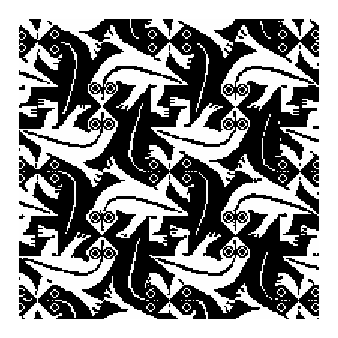
\includegraphics[clip]{1993phy8-1.eps}}
  \end{center}
\end{subquestions}
\end{question}
\begin{answer}{専攻 問題8}{}

\begin{subanswers}
\SubAnswer
  並進対称性\quad 2回回転対称性

\SubAnswer
  生体内において、アミノ酸はL型、D型のうちL型のみ存在する。また、
  蛋白質の二次構造である$\alpha-$ヘリックスは生体内では右巻きのもの
  しか存在しない。これらの蛋白質構成要素である分子に鏡映や反転対称性
  がないことは、これらの対称性を持つ分子が、生体内に存在しないことを
  示している。\\
  よって、タンパク質分子やその結晶には鏡映$\cdot$反転対称性はない。
  ($\alpha-$ヘリックスが右巻きしか存在しないのは、アミノ酸がL型
  しかないことによる。)

\SubAnswer

  \begin{subsubanswers}
  \SubSubAnswer
%    複素平面内で、$F_H,F,f_H$をvectorのように考える。これらのベクトル
%    の相対的な位置関係が分かれば良い。わかっている情報はベクトルの
%    大きさと$F_H=F+f_H$である。
%
%    \begin{center}
%      \fbox{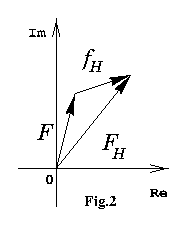
\includegraphics[clip]{1993phy8-2.eps}}
%    \end{center}
%
%    まず、原点を中心に、半径$|F_H|$の円を描く。相対的な位置関係(位相差)
%    が知りたいので、原点から大きさ$|f_H|$の円を描き、初めに描いた円と
%    の交点を求めると、その交点は$F_H=F+f_H$を満たす点である。こうして、
%    $F$の位相に関する情報が得られる。(これをArgand作図という。)
\parbox[t]{100mm}{
X線回折で観測結果として得られるのは、$|F|^2$,$|F_H|^2$,$f_H$の3つである。$f_H$は、差パターソン関数の原理により、$|F|^2$,$|F_H|^2$の2つから得られるのだが、この問題は、すでに$f(x_1,x_2,x_3)$として与えられていて、それを用いて良いと思われる。

さて、$F$,$F_H$,$f_H$は、
\begin{equation}
F_H=F+f_H \eqname{A1}
\end{equation}
の関係にあるが、これを複素平面で図示するとFig.3の様になっている。
\eqhref{A1}より$F=F_H-f_H$であるから、$F$の位相は分からないが、$-f_H$の終点(矢印の先端という意味)から、半径$|F_H|$のところのどこかにあることが分かる。また、当然、$F$は複素平面原点から半径$|F|$の円周上にある。ゆえ、この2円周の2交点A,Bのどちらか1ヶ所が$F$の値であることが分かる。

{\bf{[注]}} Fig.4(●はソーキング(付着)した重原子)の(a)(b)を比較して、(c)を理解するという方法を、解析的に取り扱う。X線回折で得られるのは、問題にもある$F(x,y,z)$だけである。いま、パターソン座標空間$(u,v,w)$を考える。(これは単位格子と同じ座標にとる。)
\[ P(u,v,w)=\frac{1}{V}\sum_{X,Y,Z \in \rm{Unit Cell}}|F(X,Y,Z)|^2 e^{-2\pi i(Xu+Yv+Zw)}\]
}\parbox[t]{60mm}{
\begin{center}
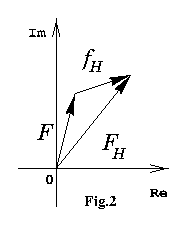
\includegraphics[clip]{1993phy8-2.eps}

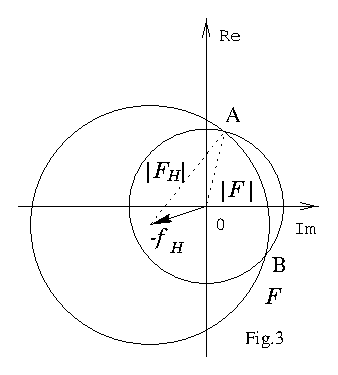
\includegraphics[clip]{1993phy8-3.eps}
\end{center}}

が各$(u,v,w)$点について計算され、3次元のパターソン関数が得られる。単位胞中の原子$i,j$の原子番号を$f_i,f_j$とすると、パターソン図上で$i,j$の原子間に相当する位置に$f_i\times f_j$の高さのピークが現れる。よって、$f_i,f_j$とともに大きい数であれば、積であるため圧倒的ピーク高となる。そのピークの$(u,v,w)$を読めれば$(x_1,x_2,x_3)$も求まる。いま、重原子同形置換法では、$|F|,|F_H|$はわかる。そこで、$(|F_H|^2 -|F|^2)=(\Delta F)^2$を係数としてパターソン関数を計算すれば、$(\Delta F)^2$には重原子の位置に関する情報が含まれているので、重原子の位置が分かるのである。これを差パターソン関数の原理と呼ぶ。

\begin{center}
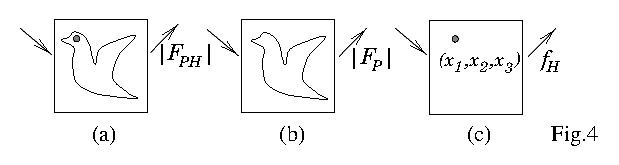
\includegraphics[clip]{1993phy8-4.eps}
\end{center}

  \SubSubAnswer 
    前問より交点は二つ存在することがわかる。よって
    $|F|^2$と$|F_H|^2$の情報からは位相角を一つの値に限定することはでき
    ない。別の場所に重原子を付加した結晶パターンから、またArgand作図を
    行ない、$F=F_H'-f_H'$となる点を求めると、また二つの交点が出るが、
    このうち一つは、前問のAまたはBのどちらかと交わる。その点が求める位
    相角である。

  \end{subsubanswers}
\end{subanswers}
\end{answer}


\end{document}
